\iffalse
\documentclass[12pt]{article}
\usepackage{graphicx}
\usepackage{amsmath}

\begin{document}
\begin{center}
\textbf\large{CHAPTER-7 \\ COORDINATE GEOMETRY}

\end{center}
\section*{Excercise 7.4}
\fi
%\begin{enumerate}[label=\thechapter.\arabic*,ref=\thechapter.\theenumi]
\begin{enumerate}[label=\thesection.\arabic*,ref=\thesection.\theenumi]
\numberwithin{equation}{enumi}
\numberwithin{figure}{enumi}
\numberwithin{table}{enumi}
\item Determine the ratio in which the line $2x+y  - 4=0$ divides the line segment joining the points $\vec{A}(2, - 2)$  and  $\vec{B}(3, 7)$.
\item Find a relation between $x$ and $y$ if the points $(x, y), (1, 2)$  and  $(7, 0)$ are collinear.

\item Find the centre of a circle passing through the points $(6, – 6), (3, – 7)$ and $ (3, 3)$.

\item The two opposite vertices of a square are $(–1, 2)$  and $ (3, 2)$. Find the coordinates of the other two vertices.
\\
	\iffalse
\documentclass[12pt]{article}
\usepackage{graphicx}
\usepackage{amsmath}
\usepackage{mathtools}
\usepackage{gensymb}

\newcommand{\mydet}[1]{\ensuremath{\begin{vmatrix}#1\end{vmatrix}}}
\providecommand{\brak}[1]{\ensuremath{\left(#1\right)}}
\providecommand{\norm}[1]{\left\lVert#1\right\rVert}
\newcommand{\solution}{\noindent \textbf{Solution: }}
\newcommand{\myvec}[1]{\ensuremath{\begin{pmatrix}#1\end{pmatrix}}}
\let\vec\mathbf

\begin{document}
\begin{center}
\textbf\large{CHAPTER-7 \\ COORDINATE GEOMETRY}

\end{center}
\section*{Excercise 7.4}

Q4.The two opposite vertices of a square are $(–1, 2) \text{ and } (3, 2)$. Find the coordinates of the other two vertices.\\
\fi
\solution
Let
\begin{align}
\vec{A} = \myvec
{
-1 \\
 2\\
},
\vec{C} = 
\myvec
{
3\\
2\\
}
\end{align}

\begin{figure}[!h]
	\begin{center} 
	    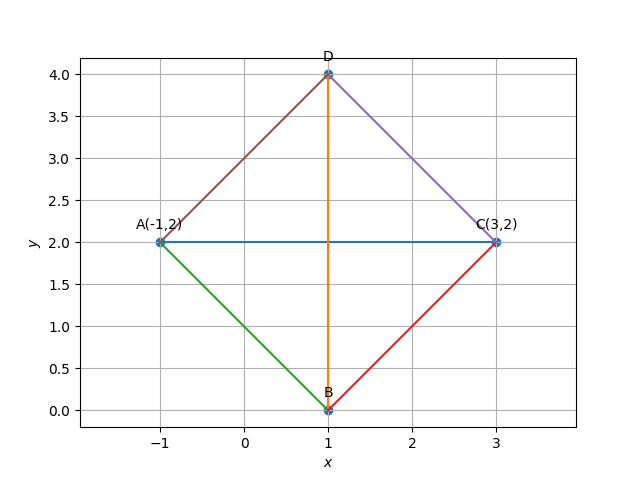
\includegraphics[width=\columnwidth]{chapters/10/7/4/4/figs/square}
	\end{center}
\caption{}
\label{fig:7/4/4/4Fig1}
\end{figure}

Shifting $\vec{A}$ to origin with reference to Fig. \ref{fig:7/4/4/4Fig2},
\begin{align}
\vec{A^{\prime}} =
\myvec{
0 \\
0\\
},
\vec{C^{\prime}} = \vec{C}-\vec{A} = 
\myvec{
4 \\
0\\
}
\end{align}

\begin{figure}[!h]
	\begin{center} 
	    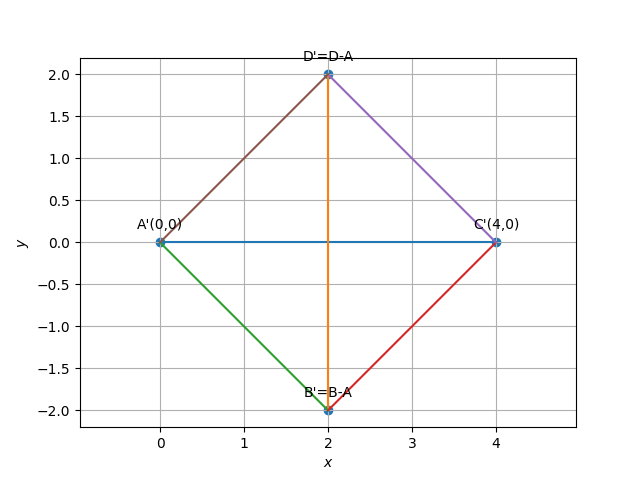
\includegraphics[width=\columnwidth]{chapters/10/7/4/4/figs/square1}
	\end{center}
\caption{}
\label{fig:7/4/4/4Fig2}
\end{figure}
\iffalse
In general,
the angle made by $AC$ with the x-axis is 
		\begin{align}
\beta = \theta + 45\degree
		\end{align}
\fi
Since
\begin{align}
\vec{C} - \vec{A} = \myvec{
4\\
0
} \equiv 
\myvec{
1\\
0
},
	\tan\theta&= \frac{0}{4} \implies 
\theta= 0\degree
\end{align}
		where
$\theta$ is the angle made by $AC$ with the x-axis.
Considering the rotation matrix 
\begin{align}
\vec{P} =
\myvec{
\cos\brak{\frac{\pi}{4}-\theta} & -\sin\brak{\frac{\pi}{4}-\theta} \\
\sin\brak{\frac{\pi}{4}-\theta} & \cos\brak{\frac{\pi}{4}-\theta} 
}
\end{align}
\iffalse
from Fig. \ref{fig:7/4/4/4Fig3},
\begin{align}
\vec{C^{\prime \prime}} = \vec{P}^\top (\vec{C}-\vec{A}) =
\myvec{
\frac{1}{\sqrt{2}} & -\frac{1}{\sqrt{2}} \\
\frac{1}{\sqrt{2}} & \frac{1}{\sqrt{2}}\\
}
\myvec{
4 \\
0\\
} = 
\myvec{
\frac{4}{\sqrt{2}} \\
\frac{4}{\sqrt{2}}\\
}
\end{align}
\begin{align}
\vec{B^{\prime \prime}} = \myvec{
 1&0\\
 0&0\\
}\vec{C^{\prime \prime}}=
\myvec{
 \frac{4}{\sqrt{2}}\\
 0\\
},
\vec{D^{\prime \prime}} = \myvec{
 0&0\\
 0&1\\
}\vec{C^{\prime \prime}}=
\myvec{
 0\\
 \frac{4}{\sqrt{2}}\\
} \text{ and }
\vec{A^{\prime \prime}} =
\myvec{
0 \\
0\\
}
\end{align}
\fi
\begin{figure}[!h]
	\begin{center} 
	    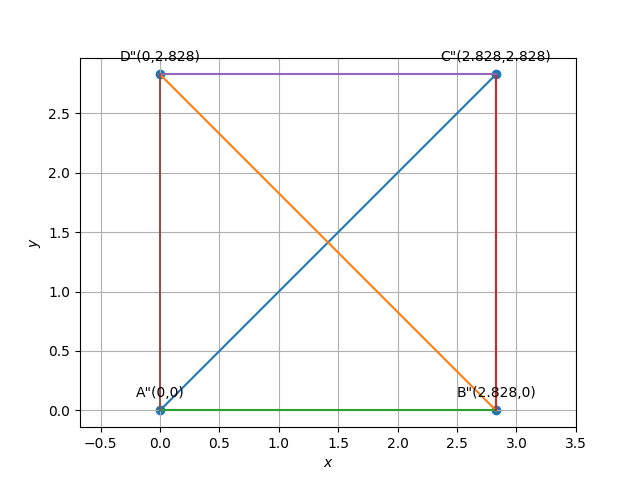
\includegraphics[width=\columnwidth]{chapters/10/7/4/4/figs/square2}
	\end{center}
\caption{}
\label{fig:7/4/4/4Fig3}
\end{figure}

\newpage
\iffalse
Again tranforming(rotating) the coordinates back to the original axis.

We know for anti-clockwise direction the rotation matrix is given as
\begin{align}
\vec{P} =
\myvec{
\cos\theta & -\sin\theta \\
\sin\theta & \cos\theta \\
}
\end{align}

Again we know that the angle is negative so the rotation will be in clockwise direction. So now the transformed(rotated) coordinates $\vec{B} \text{ and } \vec{D}$ are with refrence to 
\fi
from Figure 
%\ref{fig:7/4/4/4Fig4},
\ref{fig:7/4/4/4Fig3},
\begin{align}
	\vec{C^{\prime \prime}} &= \vec{P} (\vec{C}-\vec{A}) 
	\\
\label{eq:7/4/4/4bp}
	\vec{B^{\prime \prime}} &= \myvec{\vec{e}_1 & \vec{0}}\vec{C^{\prime \prime}}
	\\
\label{eq:7/4/4/4dp}
	\vec{D^{\prime \prime}} &= \myvec{ \vec{0} & \vec{e}_2}\vec{C^{\prime \prime}}
\end{align}
Now, 
\begin{align}
\label{eq:7/4/4/4b}
	\vec{B} = \vec{P}^{\top}\vec{B}^{\prime \prime}+\vec{A}
	\\
\label{eq:7/4/4/4d}
	\vec{D} = \vec{P}^{\top}\vec{D}^{\prime \prime}+\vec{A}
\end{align}
by reversing the process of translation and rotation.  Thus, 
from
\eqref{eq:7/4/4/4b}
\eqref{eq:7/4/4/4bp},
\eqref{eq:7/4/4/4d}
and
\eqref{eq:7/4/4/4dp}
\begin{align}
	\vec{B} = \vec{P}^{\top}\myvec{\vec{e}_1 & \vec{0}}\vec{P} (\vec{C}-\vec{A}) +\vec{A}
	\\
	\vec{D} = \vec{P}^{\top}\myvec{\vec{0} & \vec{e}_2  }\vec{P} (\vec{C}-\vec{A}) +\vec{A}
%	\vec{B} &= \brak{(\vec{C}-\vec{A})^{\top}\vec{P}^{\top} \vec{e}_1}\vec{P}^{\top}\vec{e}_1+\vec{A}
%	\\
%	\vec{D} &= \brak{(\vec{C}-\vec{A})^{\top}\vec{P}^{\top} \vec{e}_2}\vec{P}^{\top}\vec{e}_2+\vec{A}
\end{align}
yielding
		\begin{align}
\vec{B}=
\myvec{
1\\
0
},
\vec{D}
\myvec{
1\\
4
}.
		\end{align}
\iffalse
\begin{align}
\vec{B^{\prime}} &= \vec{P}\vec{B^{\prime \prime}} = \myvec{
\frac{1}{\sqrt{2}} & \frac{1}{\sqrt{2}} \\
-\frac{1}{\sqrt{2}} & \frac{1}{\sqrt{2}}\\
}
\myvec{
 \frac{4}{\sqrt{2}}\\
 0\\
} = 
\myvec{
2 \\
-2\\
}\\
\vec{D^{\prime}} &= \vec{P}\vec{D^{\prime \prime}} = \myvec{
\frac{1}{\sqrt{2}} & \frac{1}{\sqrt{2}} \\
-\frac{1}{\sqrt{2}} & \frac{1}{\sqrt{2}}\\
}
\myvec{
 0\\
 \frac{4}{\sqrt{2}}\\
} = 
\myvec{
2 \\
2 \\
}
\end{align}

\begin{figure}[!h]
	\begin{center} 
	    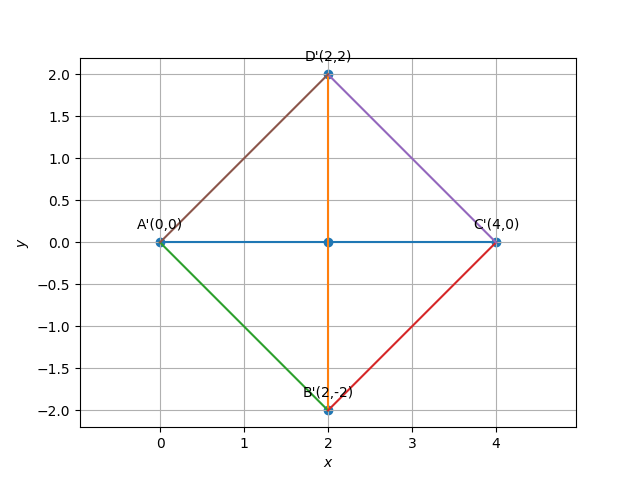
\includegraphics[width=\columnwidth]{chapters/10/7/4/4/figs/square3}
	\end{center}
\caption{}
\label{fig:7/4/4/4Fig4}
\end{figure}

Again transforming(shifting) the axis back to the original with refrence to Figure \ref{fig:7/4/4/4Fig5}
\begin{align}
\vec{B} &= \vec{B^{\prime}}+\vec{A} = \myvec{
2 \\
-2\\
}+\myvec{
-1 \\
2\\
} = 
\myvec{
1 \\
0\\
}\\
\vec{D} &= \vec{D^{\prime}}+\vec{A} = \myvec{
2 \\
2\\
}+\myvec{
-1 \\
2\\
} = 
\myvec{
1 \\
4 \\
}
\end{align}

Hence, the other two vertices are $\vec{B}(1,0) \text{ and } \vec{D}(1,4)$   

\begin{figure}[!h]
	\begin{center} 
	    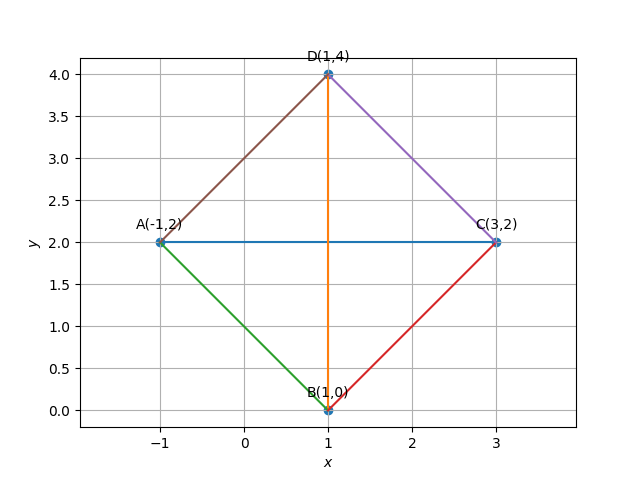
\includegraphics[width=\columnwidth]{chapters/10/7/4/4/figs/square4}
	\end{center}
\caption{}
\label{fig:7/4/4/4Fig5}
\end{figure}
which can also be expressed as
\begin{align}
\vec{B} &= \vec{A} + \vec{P}\myvec{
\vec{e_{1}}&\vec{0}\\
}
\vec{P}^\top \brak{\vec{C}-\vec{A}}\\
\vec{D} &= \vec{A} + \vec{P}\myvec{
\vec{0}&\vec{e_{2}}\\
}
\vec{P}^\top \brak{\vec{C}-\vec{A}}\\
\end{align}
where $\vec{P}$ is the rotation matrix and $\vec{A} \text{ and } \vec{C}$ are the position vectors of opposite vertices.

Derivation of the above formulas:

We know that after shifting the axis and rotating by the required angle any arbitrary square will be aligned with the x and y axis so that we can directly get the vectors $\vec{B} \text{ and } \vec{D}$ as follows
\begin{align}
\vec{C^{\prime\prime}} &= \vec{P}^\top \brak{\vec{C} - \vec{A}}\\
\vec{B^{\prime\prime}} &= \myvec{
\vec{e_{1}} & \vec{0}
}\vec{C^{\prime\prime}} = \myvec{
\vec{e_{1}} & \vec{0}
}\vec{P}^\top \brak{\vec{C} - \vec{A}}\\
\vec{B^{\prime}} &= \vec{P} \vec{B^{\prime\prime}}  = \vec{P}\myvec{
\vec{e_{1}} & \vec{0}
}\vec{P}^\top \brak{\vec{C} - \vec{A}}\\
\vec{B} &= \vec{A}+\vec{B^{\prime}}\\
 &= \vec{A} + \vec{P}\myvec{
\vec{e_{1}}&\vec{0}\\
}
\vec{P}^\top\brak{\vec{C}-\vec{A}}
\end{align}

Similarly for D it can be derived as
\begin{align}
\vec{C^{\prime\prime}} &= \vec{P}^\top \brak{\vec{C} - \vec{A}}\\
\vec{D^{\prime\prime}} &= \myvec{
\vec{0} & \vec{e_{2}}
}\vec{C^{\prime\prime}} = \myvec{
\vec{0} & \vec{e_{2}}
}\vec{P}^\top \brak{\vec{C} - \vec{A}}\\
\vec{D^{\prime}} &= \vec{P} \vec{D^{\prime\prime}} = \vec{P} \myvec{
\vec{0} & \vec{e_{2}}
}\vec{P}^\top \brak{\vec{C} - \vec{A}}\\
\vec{D} &= \vec{A}+\vec{D^{\prime}}\\
 &= \vec{A} + \vec{P}\myvec{
\vec{0}&\vec{e_{2}}\\
}
\vec{P}^\top\brak{\vec{C}-\vec{A}}
\end{align}


Verification of the above formula for the given question

\begin{align}
\vec{B} &= \myvec{
-1\\
2\\
}+\myvec{
\frac{1}{\sqrt{2}} & \frac{1}{\sqrt{2}} \\
-\frac{1}{\sqrt{2}} & \frac{1}{\sqrt{2}}\\
}\myvec{
 1&0\\
 0&0\\
}\myvec{
\frac{1}{\sqrt{2}} & -\frac{1}{\sqrt{2}} \\
\frac{1}{\sqrt{2}} & \frac{1}{\sqrt{2}}\\
}\myvec{
4\\
0\\
}\\
 &= \myvec{
-1\\
2\\
}+\myvec{
\frac{1}{\sqrt{2}} & \frac{1}{\sqrt{2}} \\
-\frac{1}{\sqrt{2}} & \frac{1}{\sqrt{2}}\\
}\myvec{
 1&0\\
 0&0\\
}\myvec{
\frac{4}{\sqrt{2}}\\
\frac{4}{\sqrt{2}}\\
}\\
 &= \myvec{
-1\\
2\\
}+\myvec{
\frac{1}{\sqrt{2}} & \frac{1}{\sqrt{2}} \\
-\frac{1}{\sqrt{2}} & \frac{1}{\sqrt{2}}\\
}\myvec{
\frac{4}{\sqrt{2}}\\
0\\
}\\
 &= \myvec{
-1\\
2\\
}+\myvec{
2\\
-2\\
}\\
 &= \myvec{
1\\
0\\
}\\
\vec{D} &= \myvec{
-1\\
2\\
}+\myvec{
\frac{1}{\sqrt{2}} & \frac{1}{\sqrt{2}} \\
-\frac{1}{\sqrt{2}} & \frac{1}{\sqrt{2}}\\
}\myvec{
 0&0\\
 0&1\\
}\myvec{
\frac{1}{\sqrt{2}} & -\frac{1}{\sqrt{2}} \\
\frac{1}{\sqrt{2}} & \frac{1}{\sqrt{2}}\\
}\myvec{
4\\
0\\
}\\
 &= \myvec{
-1\\
2\\
}+\myvec{
\frac{1}{\sqrt{2}} & \frac{1}{\sqrt{2}} \\
-\frac{1}{\sqrt{2}} & \frac{1}{\sqrt{2}}\\
}\myvec{
 0&0\\
 0&1\\
}\myvec{
\frac{4}{\sqrt{2}}\\
\frac{4}{\sqrt{2}}\\
}\\
 &= \myvec{
-1\\
2\\
}+\myvec{
\frac{1}{\sqrt{2}} & \frac{1}{\sqrt{2}} \\
-\frac{1}{\sqrt{2}} & \frac{1}{\sqrt{2}}\\
}\myvec{
0\\
\frac{4}{\sqrt{2}}\\
}\\
 &= \myvec{
-1\\
2\\
}+\myvec{
2\\
2\\
}\\
 &= \myvec{
1\\
4\\
}
\end{align}
\fi








\iffalse
\item The Class X students of a secondary school in Krishinagar have been allotted a rectangular plot of land for their gardening activity. Sapling of Gulmohar are planted on the boundary at a distance of 1m from each other. There is a triangular grassy lawn in the plot as shown in fig.\ref{fig:Fig1}. The students are to sow seeds of flowering plants on the remaining area of the plot.\\

\begin{figure}[!h]
	\begin{center} 
	    \includegraphics[width=\columnwidth]{./ss}
	\end{center}
\caption{}
\label{fig:Fig1}
\end{figure}
\item Taking $\vec{A}$ as origin, find the coordinates of the vertices of the triangle.
\item What will be the coordinates of the vertices of $\triangle PQR$ if $\vec{C}$ is the origin?
Also calculate the areas of the triangles in these cases. What do you observe?
\end{enumerate}

\fi

\item The vertices of a $\triangle ABC$ are $\vec{A}(4,6), \vec{B}(1,5)$ and  $\vec{C}(7,2)$. A line is drawn to intersect sides $AB$ and $AC$ at $\vec{D}$ and $\vec{E}$ respectively, such that $\frac{AD}{AB} = \frac{AE}{AC} = \frac{1}{4}$. Calculate the area of $\triangle ADE$ and compare it with the area of the $\triangle ABC$.

\item Let $\vec{A}(4, 2), \vec{B}(6, 5)$  and $ \vec{C}(1, 4)$ be the vertices of $\triangle ABC$.

\begin{enumerate}
\item The median from $\vec{A}$ meets $BC$ at $\vec{D}$. Find the coordinates of the point $\vec{D}$.
\item Find the coordinates of the point $\vec{P}$ on $AD$ such that $AP : PD = 2 : 1$.
\item Find the coordinates of points $\vec{Q}$ and $\vec{R}$ on medians $BE$ and $CF$ respectively such that $BQ : QE = 2 : 1$  and  $CR : RF = 2 : 1$.
\item What do you observe?
\item If $\vec{A}, \vec{B}$ and $\vec{C}$  are the vertices of $\triangle ABC$, find the coordinates of the centroid of the triangle.
\end{enumerate}
\solution
	\iffalse
\documentclass[12pt]{article}
\usepackage{graphicx}
\usepackage[none]{hyphenat}
\usepackage{graphicx}
\usepackage{listings}
\usepackage[english]{babel}
\usepackage{graphicx}
\usepackage{caption} 
\usepackage{booktabs}
\usepackage{array}
\usepackage{amssymb} % for \because
\usepackage{amsmath}   % for having text in math mode
\usepackage{extarrows} % for Row operations arrows
\usepackage{listings}
\usepackage[utf8]{inputenc}
\lstset{
  frame=single,
  breaklines=true
}
\usepackage{hyperref}
  
%Following 2 lines were added to remove the blank page at the beginning
\usepackage{atbegshi}% http://ctan.org/pkg/atbegshi
\AtBeginDocument{\AtBeginShipoutNext{\AtBeginShipoutDiscard}}


%New macro definitions
\newcommand{\mydet}[1]{\ensuremath{\begin{vmatrix}#1\end{vmatrix}}}
\providecommand{\brak}[1]{\ensuremath{\left(#1\right)}}
\newcommand{\solution}{\noindent \textbf{Solution: }}
\newcommand{\myvec}[1]{\ensuremath{\begin{pmatrix}#1\end{pmatrix}}}
\providecommand{\norm}[1]{\left\lVert#1\right\rVert}
\providecommand{\abs}[1]{\left\vert#1\right\vert}
\let\vec\mathbf

\begin{document}

\begin{center}
\title{\textbf{VECTORS}}
\date{\vspace{-5ex}} %Not to print date automatically
\maketitle
\end{center}

\section{10$^{th}$ Maths - EXERCISE-7.4}

Let A(4, 2), B(6, 5) and C(1, 4) be the vertices of $\triangle ABC$
\begin{enumerate}
\item The median from A meets BC at D. Find the coordinates of the point D.
\item Find the coordinates of the point P on AD such that $AP : PD = 2 : 1$
\item Find the coordinates of points Q and R on medians BE and CF respectively such
that $BQ : QE = 2 : 1 \text{and} CR : RF = 2 : 1.$
\item What do yo observe?
\item If $A(x_1, y_1), B(x_2, y_2) \text{and} C(x_3, y_3)$ are the vertices of $\triangle ABC$, find the coordinates of the centroid of the triangle.
\end{enumerate}

Given points are
\begin{align}
\vec{A}=\myvec{4\\ 2} ,
\vec{B}=\myvec{6\\ 5} ,
\vec{C}=\myvec{1\\ 4}
\end{align}
\fi

\begin{enumerate}
\item 
\begin{align}
\vec{D}&=\frac{\vec{B}+\vec{C}}{2}\\
&=\myvec{\frac{7}{2}\\[2pt] \frac{9}{2}}\\
\vec{E}&=\frac{\vec{A}+\vec{C}}{2}\\
&=\myvec{\frac{5}{2}\\ 3}\\
\vec{F}&=\frac{\vec{A}+\vec{B}}{2}\\
&=\myvec{5\\ \frac{7}{2}}
\end{align}

\item 
	For
$n=2$,
\begin{align}
\vec{P}&=\frac{1}{1+n}\brak{\myvec{\vec{A}+n\vec{D}}}\\
&=\frac{1}{3}\myvec{11\\11}
\end{align}

\item 
\begin{align}
\vec{Q}&=\frac{1}{1+n}\brak{\myvec{\vec{B}+n\vec{E}}}\\
&=\frac{1}{3}\myvec{11\\11}\\
\vec{R}&=\frac{1}{1+n}\brak{\myvec{\vec{C}+n\vec{F}}}\\
&=\frac{1}{3}\myvec{11\\11}\\
\end{align}

\item 
 $\vec{P},\vec{Q},\vec{R}$ are the same point.
   
\item 
\begin{align}
\vec{G}&=\frac{\vec{D}+\vec{E}+\vec{F}}{3}\\
&=\frac{1}{3}\myvec{11\\11}\\
\end{align} 
\end{enumerate}
See Fig.  
  \ref{fig:chapters/10/7/4/7/Figure}.
\begin{figure}[h!]
\centering
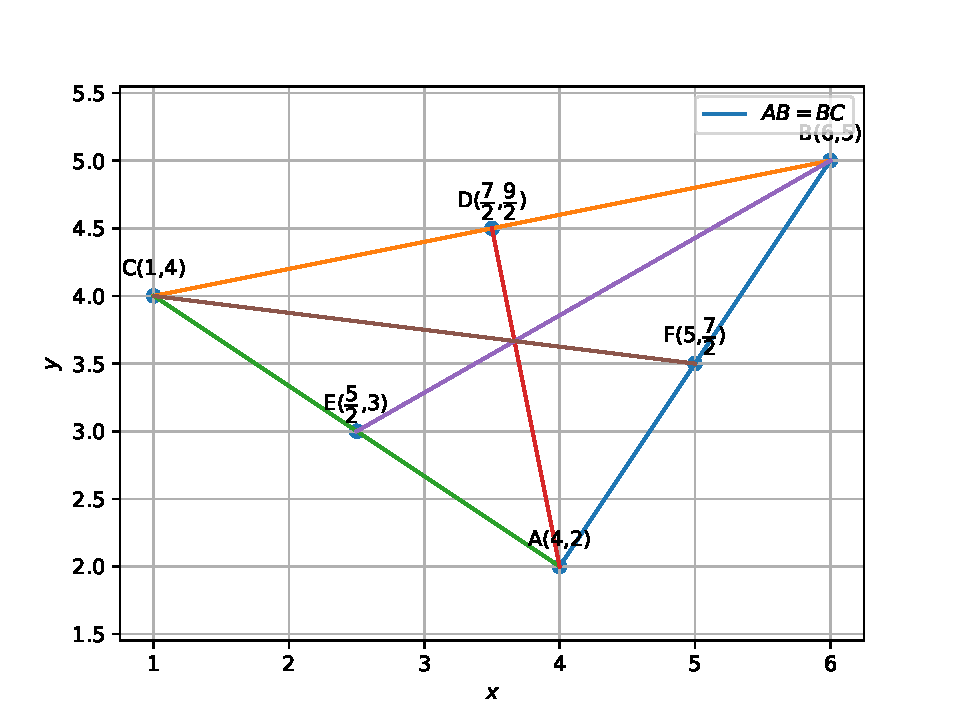
\includegraphics[width=\columnwidth]{chapters/10/7/4/7/figs/dj.pdf}
\caption{}
  \label{fig:chapters/10/7/4/7/Figure}
\end{figure}



\item $ABCD$ is a rectangle formed by the points $\vec{A}(–1, –1), \vec{B}(– 1, 4), \vec{C}(5, 4)$  and  $\vec{D}(5, – 1)$. $\vec{P}, \vec{Q}, \vec{R}$ and $\vec{S}$ are the mid-points of $AB, BC, CD$ and $DA$ respectively. Is the quadrilateral $PQRS$ a square? a rectangle? or a rhombus? Justify your answer.
	\\
	\iffalse
\documentclass[12pt]{article}
\usepackage{graphicx}
%\documentclass[journal,12pt,twocolumn]{IEEEtran}
\usepackage[none]{hyphenat}
\usepackage{graphicx}
\usepackage{listings}
\usepackage[english]{babel}
\usepackage{graphicx}
\usepackage{caption} 
\usepackage{hyperref}
\usepackage{booktabs}
\usepackage{array}
\usepackage{amsmath}   % for having text in math mode
\usepackage{listings}
\lstset{
  frame=single,
  breaklines=true
}
  
%Following 2 lines were added to remove the blank page at the beginning
\usepackage{atbegshi}% http://ctan.org/pkg/atbegshi
\AtBeginDocument{\AtBeginShipoutNext{\AtBeginShipoutDiscard}}
%


%New macro definitions
\newcommand{\mydet}[1]{\ensuremath{\begin{vmatrix}#1\end{vmatrix}}}
\providecommand{\brak}[1]{\ensuremath{\left(#1\right)}}
\providecommand{\norm}[1]{\left\lVert#1\right\rVert}
\newcommand{\solution}{\noindent \textbf{Solution: }}
\newcommand{\myvec}[1]{\ensuremath{\begin{pmatrix}#1\end{pmatrix}}}
\let\vec\mathbf

\begin{document}

\begin{center}
\title{\textbf{Properties of Quadrilaterals}}
\date{\vspace{-5ex}} %Not to print date automatically
\maketitle
\end{center}

\setcounter{page}{1}



\section{10$^{th}$ Maths - Chapter 7}

This is Problem-8 from Exercise 7.4

\begin{enumerate}
\item ABCD is a rectangle formed by the points $\vec{A}(–1, –1), \vec{B}(– 1, 4), \vec{ C}(5, 4) \text{ and } \vec{D}(5, – 1)$. $\vec{P,Q,R} \text{ and } \vec{S}$ are the mid-points of $\vec{AB, BC, CD} \text{ and } \vec{DA}$ respectively. Is the quadrilateral
PQRS a square? a rectangle? or a rhombus? Justify your answer. \\
\fi
\solution 
See Fig. \ref{fig:10/7/4/8Fig3}.
\begin{align}
  \label{eq:10/7/4/8det2f}
  \vec{P} &= \frac{1}{2}\brak{\vec{A}+\vec{B}} =   \frac{1}{2}\brak{\myvec{
  -1 \\
  -1 \\
 } + \myvec{
  -1 \\
  4 \\
 } 
 } = \myvec{
 -1 \\
 \frac{3}{2} \\
 }   \\
 \vec{Q} &= \frac{1}{2}\brak{\vec{B}+\vec{C}} =   \frac{1}{2}\brak{\myvec{
  -1 \\
  4 \\
 } + \myvec{
  5 \\
  4 \\
 } 
 } = \myvec{
 2 \\
 4 \\
 }   \\
 \vec{R} &= \frac{1}{2}\brak{\vec{C}+\vec{D}} =   \frac{1}{2}\brak{\myvec{
  5 \\
  4 \\
 } + \myvec{
  5 \\
  -1\\
 } 
 } = \myvec{
 5 \\
 \frac{3}{2} \\
 }   \\
 \vec{S} &= \frac{1}{2}\brak{\vec{D}+\vec{A}} =   \frac{1}{2}\brak{\myvec{
  5 \\
  -1 \\
 } + \myvec{
  -1 \\
  -1\\
 } 
 } = \myvec{
 2\\
 -1 \\
 }   
\end{align}

\begin{figure}[!h]
	\begin{center}
		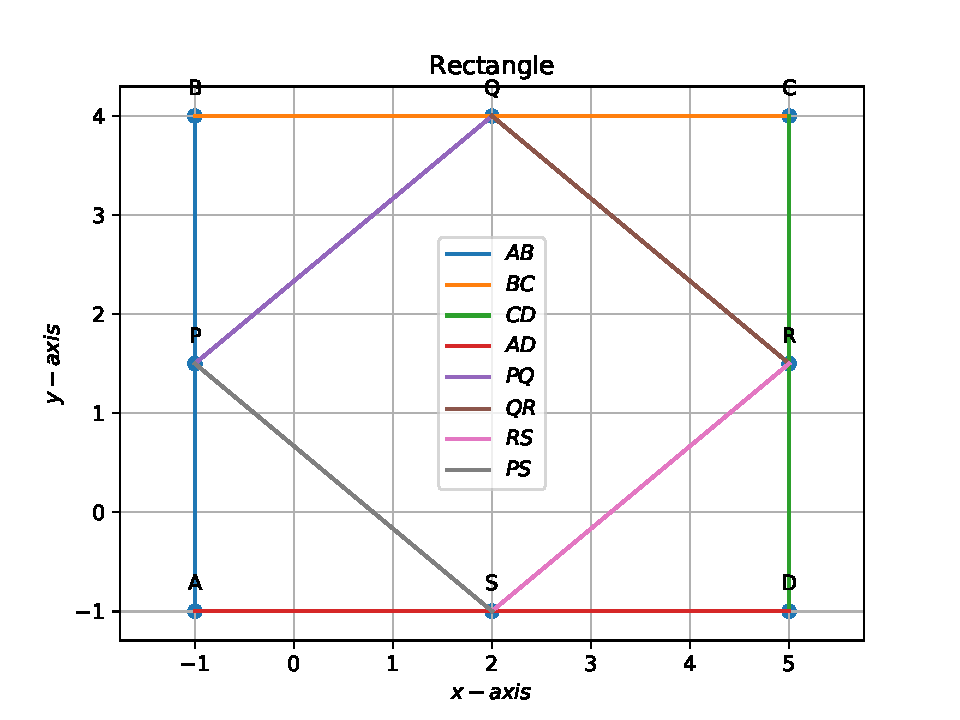
\includegraphics[width=\columnwidth]{chapters/10/7/4/8/figs/problem1.pdf}
	\end{center}
\caption{}
\label{fig:10/7/4/8Fig3}
\end{figure}
We know that PQRS is a parallelogram. To know, if it is a rectangle, we need to ascertain whether any of the two adjacent sides are perpendicular. 
That means $\brak{\vec{Q}-\vec{P}}^\top\brak{\vec{R}-\vec{Q}}$ should be equal to zero. 
\begin{align}
\vec{Q}-\vec{P} &=  \myvec{
 2 \\
 4 \\
 } - \myvec{
 -1 \\
 \frac{3}{2} \\
 } = \myvec{
 3 \\
 \frac{5}{2} \\ 
 } \\
 \vec{R}-\vec{Q} &=  \myvec{
 5 \\
 \frac{3}{2}\\
 } - \myvec{
 2 \\
 4 \\
 } = \myvec{
 3 \\
 -\frac{5}{2} \\ 
 } \\ 
 \brak{\vec{Q}-\vec{P}}^\top\brak{\vec{R}-\vec{Q}} &= \myvec{
 3 & \frac{5}{2}} \myvec{
 3 \\
 -\frac{5}{2} 
 } \neq 0
\end{align}
Therefore PQRS is not a rectangle. Let us check if it is a rhombus. For a rhombus, the diagonals bisect perpendicularly. That means $\brak{\vec{R}-\vec{P}}^\top\brak{\vec{S}-\vec{Q}}$ should be equal to zero. 
\begin{align}
\vec{R}-\vec{P} &=  \myvec{
 5 \\
 \frac{3}{2} \\
 } - \myvec{
 -1 \\
 \frac{3}{2} \\
 } = \myvec{
 6 \\
 0 \\ 
 } \\
 \vec{S}-\vec{Q} &=  \myvec{
 2 \\
 -1 \\
 } - \myvec{
 2 \\
 4 \\
 } = \myvec{
 0 \\
 -5 \\ 
 } \\ 
 \brak{\vec{R}-\vec{P}}^\top\brak{\vec{S}-\vec{Q}} &= \myvec{
 6 & 0} \myvec{
 0 \\
 -5 \\
 } = 0
\end{align}
Therefore $PQRS$ is a rhombus.




\end{enumerate}



